\chapter{Introduction}

People re-identification (Re-ID) has been an intense research topic in recent years, the main goal of which is to match an image of a given person with other images of the same person. Person Re-ID has great potential in video surveillance, target detection and tracking, and forensic search. In an intelligent 
surveillance system, suppose there are many cameras and these cameras may not have overlapping field of view, the system has to automatically identify individuals that appear in different cameras. It is quite challenging since the matching accuracy is greatly influenced by many factors like occlusion, illumination variation, camera settings and color response. Surveillance system like this can be applied to forensic search, domotics applications and distributed multi-camera surveillance system to track individuals across different cameras without overlapping field of view over time.

In Re-ID, those images with known labels are called gallery images, and the image used to determine its label is called a probe image. The probe image and gallery images can be from the same or different camera views, so the viewpoint and illumination between the probe and gallery image can be quite different. Also, because of the different color response of different cameras, the images of the same person may look different in different cameras. Occlusions between the camera and target can also bring about much difficulty.  In a word, images of the same person may look different while images of different persons may look quite the same. In Re-ID, the main goal is to improve the matching accuracy.

Given a sequence or video of individuals, there are three steps to match a person. A simple workflow is shown in Figure \ref{workflow}. However, since most Re-ID datasets are already cropped manually or by an automatic detector, most Re-ID work will only focus on robust descriptors design and efficient matching algorithm aimed at those well-cropped images. 


\begin{figure}[H]
\centering
%\begin{raggedleft}
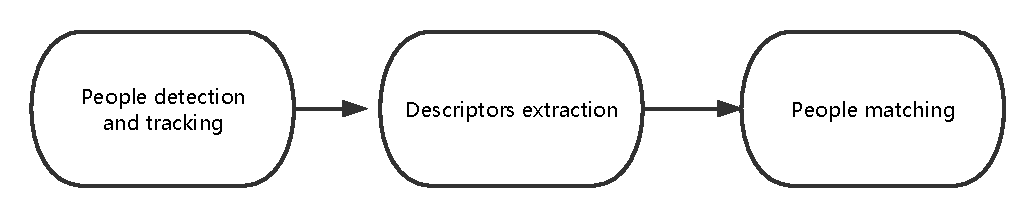
\includegraphics[scale = 0.7]{/Users/JohnsonJohnson/Downloads/thesis_1/Figures/REIDworkflow1.pdf}
%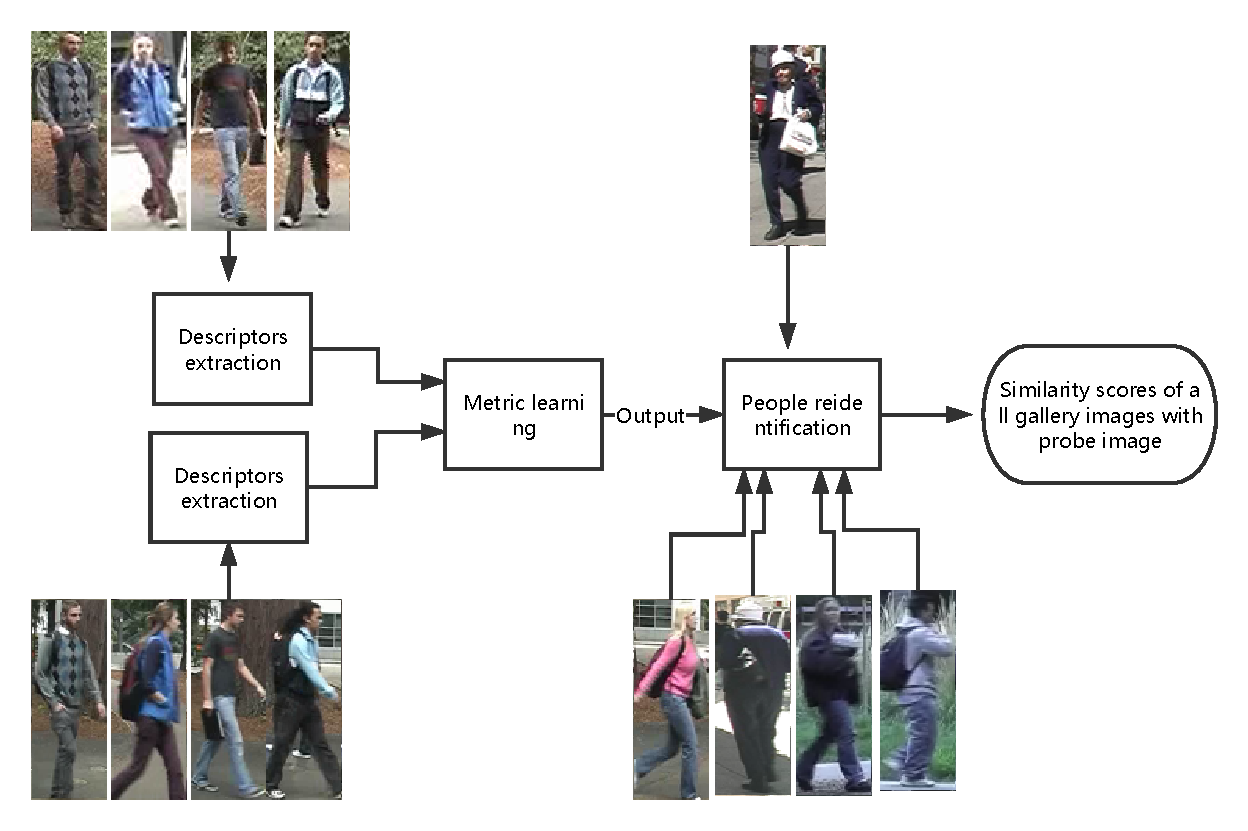
\includegraphics[width=1\linewidth]{REIDworkflow.pdf}
\vspace{1em}
\caption{Re-ID workflow}
%\end{raggedleft}
\end{figure}
\label{workflow}

\begin{figure}[H]
\centering
%\begin{raggedleft}
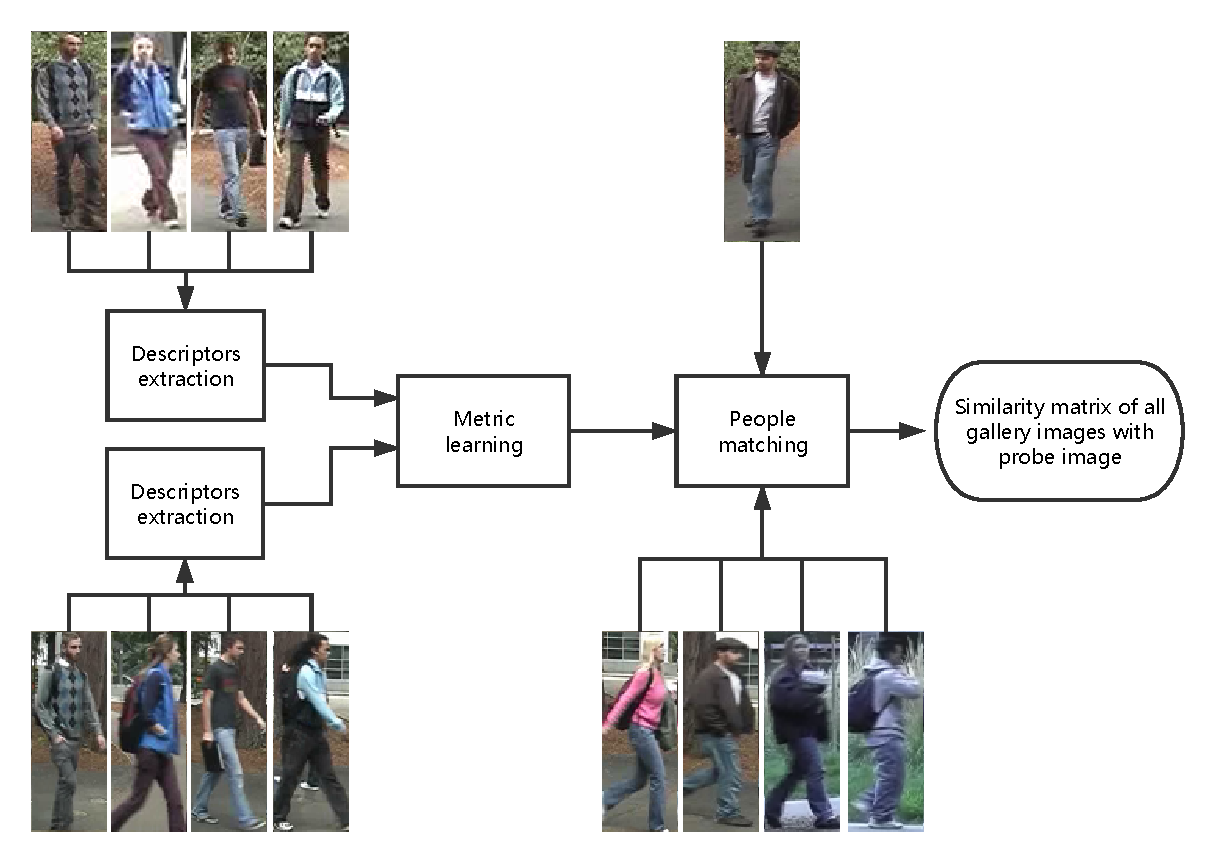
\includegraphics[scale = 0.7]{/Users/JohnsonJohnson/Downloads/thesis_1/Figures/REIDworkflow2.pdf}
%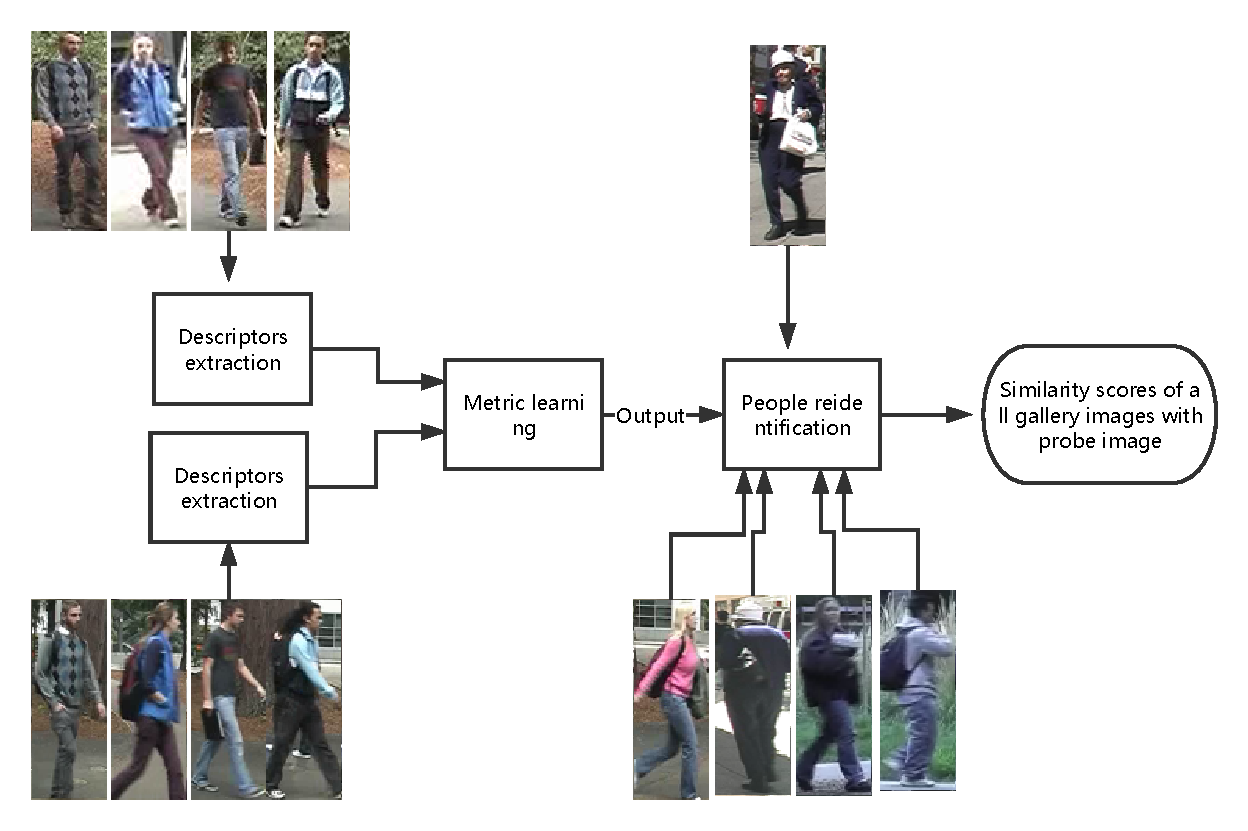
\includegraphics[width=1\linewidth]{REIDworkflow.pdf}
\vspace{1em}
\caption{A typical single-shot Re-ID workflow}
%\end{raggedleft}
\end{figure}




The first task in Re-ID is to design a robust descriptor to represent images. The descriptor is supposed to contain the key information for each captured person. Basically, the descriptors are supposed to be robust and discriminative. One straightforward way is to extract the color, textural information of images and then use descriptors to compute the similarity scores. But this method turns out to be not robust to the illumination variation, camera color response difference and camera angle settings.  Therefore, many other advanced descriptors take into account the correlation of color, texture and position together to improve performance.

The second is to design the similarity computing methodology (i.e., compare the similarity of two descriptors), which is also called distance metric learning. Metric learning can be divided into supervised and unsupervised distance metric learning \cite{MetricLearningSurvey}. The supervised distance metric requires the labels of class while the unsupervised one doesn't. Many previous supervised metric learning methods try to utilize different distance constraints to learn a Mahalanobis metric which has a form as $D(\bm{x},\bm{y}) = (\bm{x} - \bm{y})^T\bm{M}(\bm{x} - \bm{y})$. For example, in \cite{NFST} the constraint is to project all descriptors of the same class to the same point while projecting descriptors of different classes to different points in a kernel space. In \cite{TDL} the constraint is the maximal intraclass distance should be at least one unit smaller than the minimal interclass distance. In \cite{PRDC} the constraint is that the distance of negative class pair should be smaller than the positive class pairs. Different distance constraints leads to different semi-positive definite (SPD) matrix $\bm{M}$ to be learned so that $\bm{M}$ satisfies predefined constraints.

\textbf{Person detection, person re-identification and face recognition} There are a few differences between the three concepts. Person detection or pedestrian detection is to detect the presence of human body in an area of space. Person re-identification is to judge if two individuals detected in the same or different cameras are the same person. In person re-identification the person detection work must have been finished before attempting people re-identification. Face recognition is to identify a person by comparing its facial feature with a database of facial features. Face recognition is very similar with person re-identification, they all need to compare an input feature with a database of features to identify the input. However, face recognition utilizes only facial features, while person re-identification takes advantage of the whole appearance features (facial feature may be used if the image resolution is high enough). In many surveillance systems, due to the low resolution and viewpoint change, the human faces are not visible or very blurry. In this case face recognition can not be used. 


	
\section{Basic concepts}
People re-identification can be divided into a few categories according to different conditions. Some general concepts are listed below.\\
\indent \textbf{Open-set and closed-set Re-ID} \cite{REIDsurvey} According to the gallery size and how the gallery size evolves, Re-ID can be divided into open-set Re-ID and closed-set Re-ID. In closed-set Re-ID, no new identities will be added to the gallery set, and gallery size remains the same as time goes by. Furthermore, the probe set will be a subset of the gallery set. That means, the number of unique identities in the gallery set will be equal or greater than the probe set. In open-set Re-ID, the gallery set will evolve as time goes by. Each time a probe image is entered into the recognition system, the system will judge if it has a corresponding match in the gallery set. If the probe image doesn't match any of the gallery images, it will be regarded as a new identity and will be added to the gallery set. The probe set is not necessarily the subset of the gallery set. 

\textbf{Long-term and short-term Re-ID} According to the time interval between gallery and probe images, Re-ID can be divided into long-term and short-term Re-ID.  In short-term Re-ID the time interval between gallery and probe images is small, say a few minutes or several hours. Conversely, long-term Re-ID refers to the case that the time interval between gallery and probe images is a few days or even longer. One difference to consider regarding the long time interval between gallery and probe images is the variation of individuals' clothing and appearance. If the gallery images were shot a few days prior, the same individual may have changed his suit or taken off his bag, causing the appearance to change. In this case, it will be much more difficult to recognize the same identity in long-term Re-ID. In most cases, we use short-term Re-ID, which guarantees that the appearance of the same person will remain the same and we will only need to consider the differences brought by other factors such as viewpoint variation and occlusions.


\textbf{Single-shot and multi-shot Re-ID} According to the size of the sample set for each person, Re-ID can be divided into single-shot and multi-shot approaches. In single-shot Re-ID, only one image is provided for a person in a camera view. Single-shot Re-ID is challenging because only limited information can be extracted. One example is the VIPeR dataset shown in Figure \ref{VIPeRimages}. For each person in this dataset only one image is provided in each camera view, and the viewpoint of each view is different. In multi-shot Re-ID, a sequence of images is provided for a person in a camera view. Compared with single-shot Re-ID, more information, like temporal-spatial information, can be extracted from the sample set. One example of multi-shot dataset is the prid\_2011 dataset shown in Figure \ref{PRID2011images}, which provides a long sequence of images for each person in a single camera view.

%-------------------------------------------------
\begin{figure}[H]

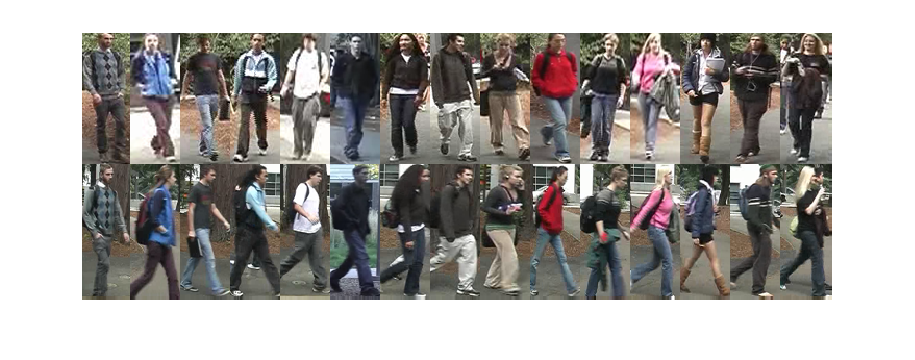
\includegraphics[width=1\linewidth]{/Users/JohnsonJohnson/Downloads/thesis_1/Figures/singleREID.eps}
\vspace{-3em}
\caption{The VIPeR dataset}
\label{VIPeRimages}
\end{figure}

%-------------------------------------------------

\begin{figure}[H]

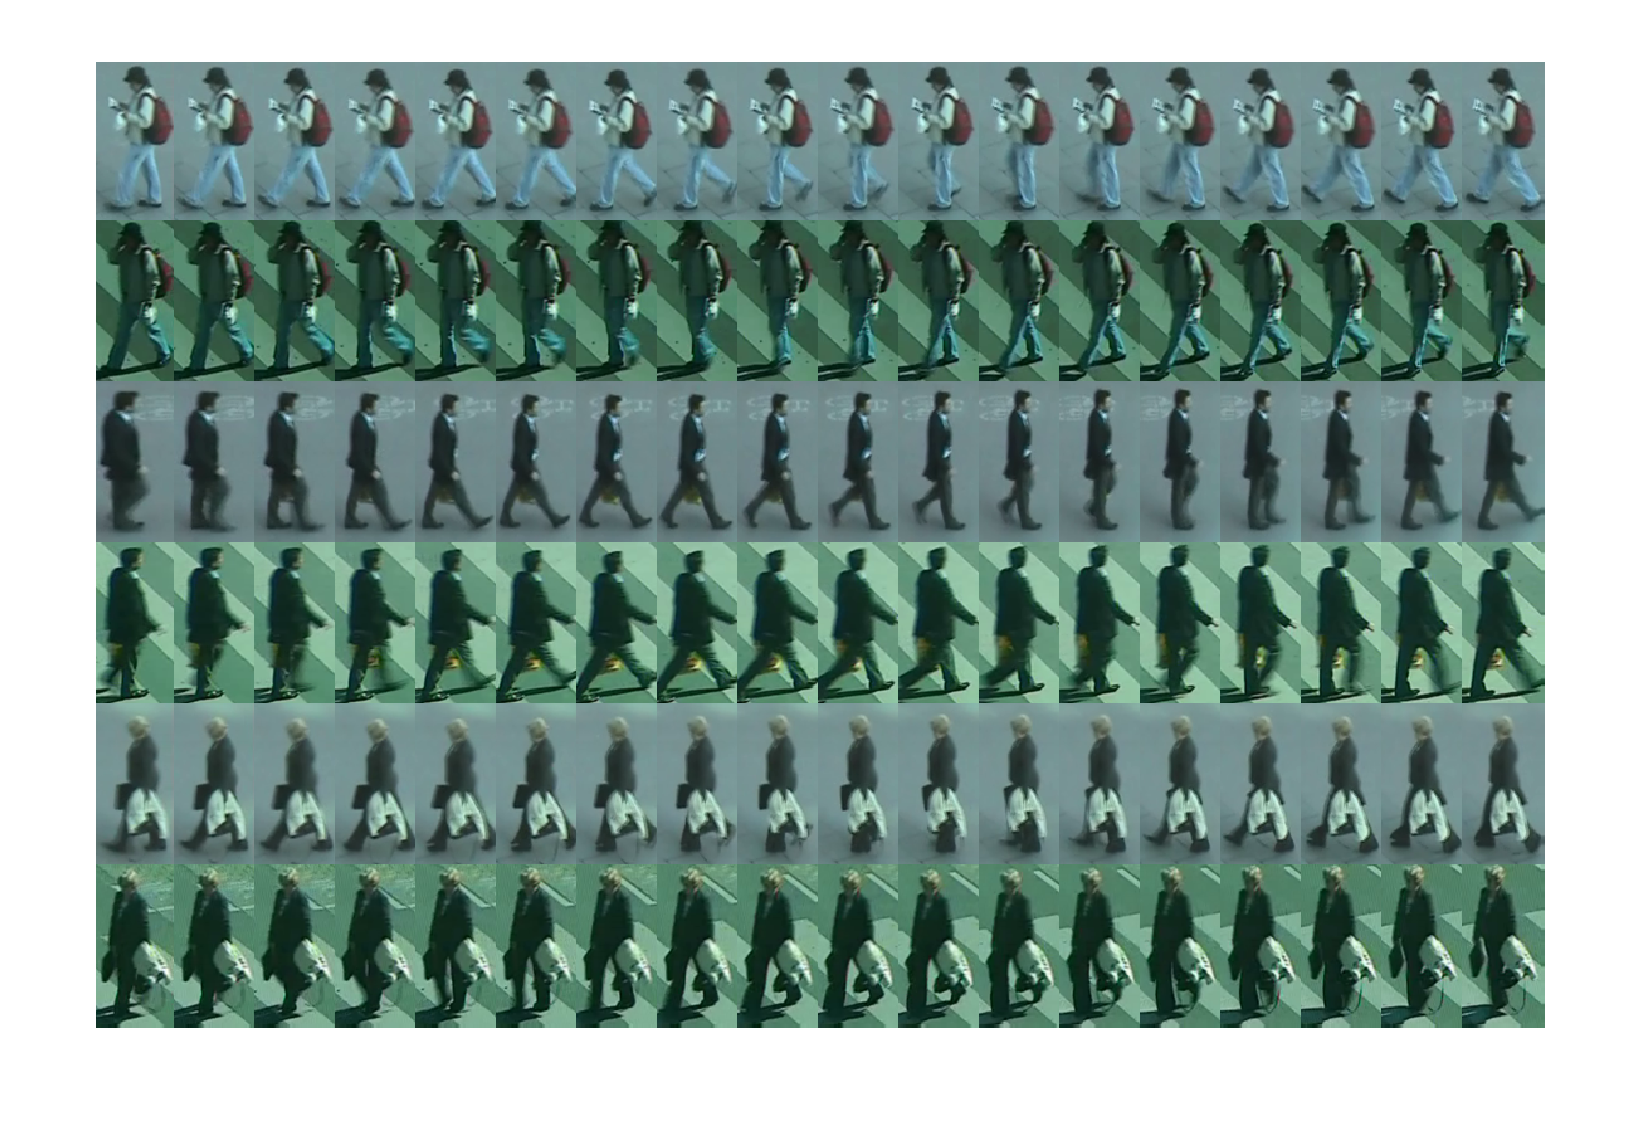
\includegraphics[width=1\linewidth]{/Users/JohnsonJohnson/Downloads/thesis_1/Figures/Multishots.eps}
\vspace{-3em}
\caption{Samples from the prid\_2011 dataset}
\label{PRID2011images}
\end{figure}

In this thesis, we use the short-term, single-shot and close-set Re-ID. We assume the Re-ID is a short-term case so that the individuals wear the same clothes. This is vital because if individuals change their clothes, it won't be valid to identify them by their appearance features. Actually in most real-time surveillance systems, individuals do wear the same clothes over the surveillance. One example is to recognize and tracking customers in a store. The customers in a store wear the same clothes through out the time.

\section{Challenges}

\textbf{Detection, tracking and dataset labelling for supervised learning} Though classical person re-identification focuses on robust descriptors design and matching algorithms, in real-time application, the detection and tracking has to be operated on video frames to get bounding boxes of individuals. A good detection and tracking algorithm is necessary for Re-ID. Furthermore, training the matching algorithm is a supervised process, thus we have to know the labels for those training data. 

\textbf{Descriptors design} Good descriptors should be robust to the variation of people's postures, outer environment changes and camera settings. Though there have been many kinds of descriptors based on different property like color and texture, it is hard to judge which property is universally useful for different camera settings. In fact, the robustness, reliability and feasibility depends on different camera settings and viewing conditions. What's more, the pedestrian background may add many errors to descriptors, so it is important to quantify the impact of a noisy background. Many works have tried to use a segmented foreground of pedestrians, so it is important to design segmentation algorithms. The automatic foreground segmentation for a single frame is difficult because there isn't much information available compared with video background segmentation. Take the VIPeR dataset as an example. There is only one frame for each view of a certain person, thus the segmented foreground masks are imperfect, and chances are high that important body parts will be lost. A segmented foreground provided by \cite{SDALF} is shown in Figure \ref{VIPeRFG}.
%-------------------------------------------------
\begin{figure}[H]
\centering
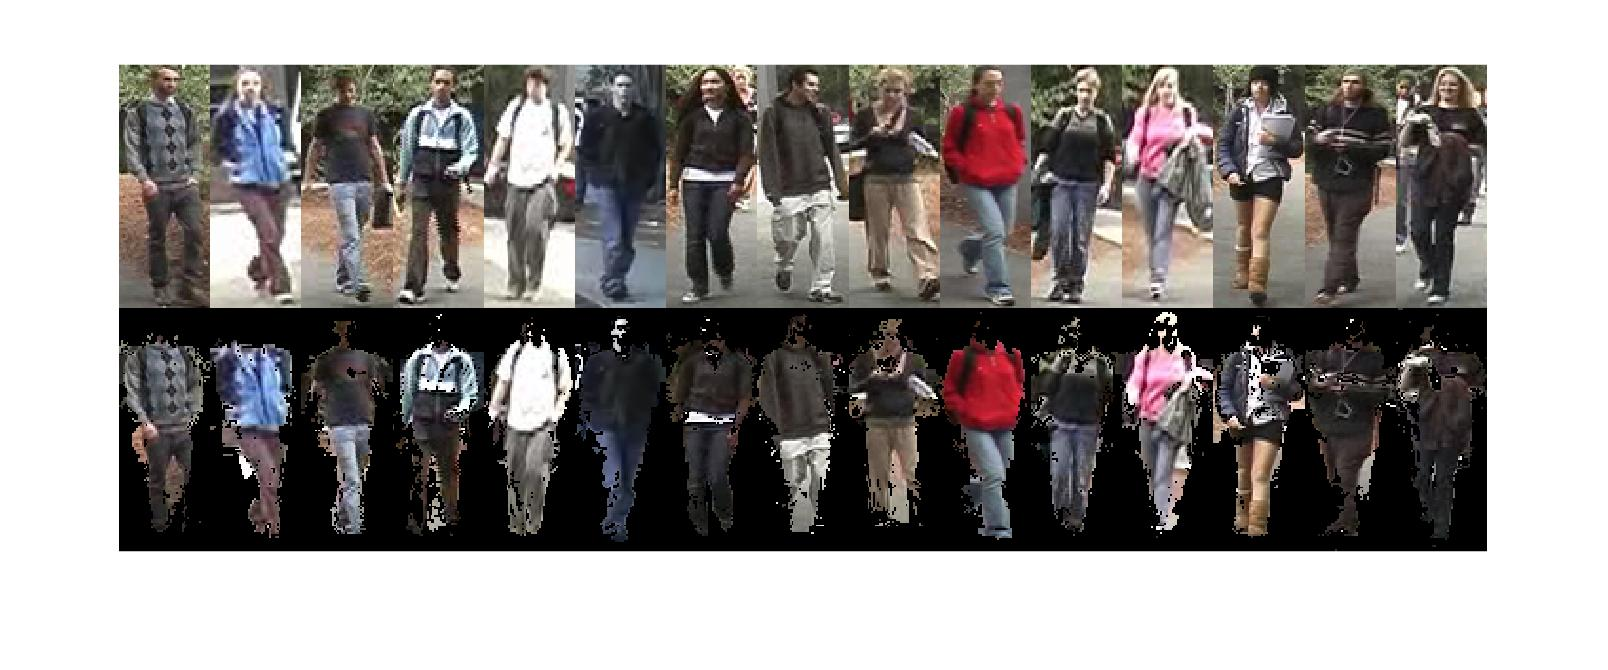
\includegraphics[width=1\linewidth]{/Users/JohnsonJohnson/Downloads/thesis_1/Figures/FGdemo.jpg}
\vspace{-3em}
\caption{VIPeR foreground}
\label{VIPeRFG}
\end{figure}

%-------------------------------------------------
\textbf{Efficient matching algorithm design} 	
When designing machine learning algorithms to match persons, there are many limitations. One of them is the small sample size problem \cite{NFST}. The extracted descriptors usually has a high dimension $d$ but only a small number of samples $n(n<<d)$, and underfitting may appear because of insufficient data samples with high dimension. It is also necessary to take into consideration intraclass and interclass distance of samples. The intraclass distance means the distance of two samples with the same class label, while interclass distance is the distance of samples with different class labels. 

\textbf{Feasibility, complexity and scalability} When applying those descriptors and matching algorithms, we have to consider real-time performance. The Re-ID datasets usually have small sample sizes, but in a surveillance network, more pedestrians in different cameras can be presented simultaneously. A system like this has plenty of individuals to re-identify, which requires that the processing time for a single probe be short for low latency. Because the gallery in this system evolves, it is crucial to design an algorithm that can determine if a person appearing in a current camera is new or has previously appeared in the gallery.

\section{My work in this thesis}

In this thesis, the programming involves C++, Matlab and Python. First the background segmentation's influence on Re-ID matching accuracy has been studied. A basic histogram descriptor is implemented with C++. By changing the color space parameters and plotting its matching accuracy curve on VIPeR dataset, the HSV color space is proved to be the best choice for histogram feature. Then by comparing the matching accuracy of HSV and other textural feature including local binary pattern (LBP) and histogram of gradient (HOG), it can be concluded that foreground segmentation (the segmentation is imperfect due to only one frame is provided for each individual) increases HSV's performance while decreases the performance of LBP and HOG. The CMC figures in chapter 3 are plotted with Python or Matlab

Second three variants of the hierarchical Gaussian descriptors have been designed and implemented with Matlab based on the source code from \cite{GOG}. After comparing their performance with the original version of hierarchical Gaussian descriptor the original version has the best performance.
 
Third, the metric learning is designed and implemented with Matlab. In many previous works, the kernel local Fisher discriminant analysis is used as a subspace learning method, and Euclidean distance is usually used in the subspace to measure similarity. In this thesis, the KLFDA \cite{KLFDA} method is used as a dimension-reducing method to project high-dimensional descriptors to a lower-dimensional space. Compared with other dimension reduction methods, KLFDA is a supervised method that takes into consideration intraclass and interclass information; therefore, less information is lost after dimension reduction. A Mahalanobis distance based matrix $\bm{M}$ is then learned based on the limitation that the distance of people from the same class should be at least one unit smaller than the distance of people from different classes. A target function that penalizes large intraclass distance and small interclass distance is created. When the target function converges by iterative computation, the matrix $\bm{M}$ is thought to be optimal. It turns out that this metric learning exhibits good performance when compared with other metric learning methods. A workflow of proposed work is in Figure \ref{ProposedWorkflow}.

%------------------------------------------------------------
\begin{figure}[H]

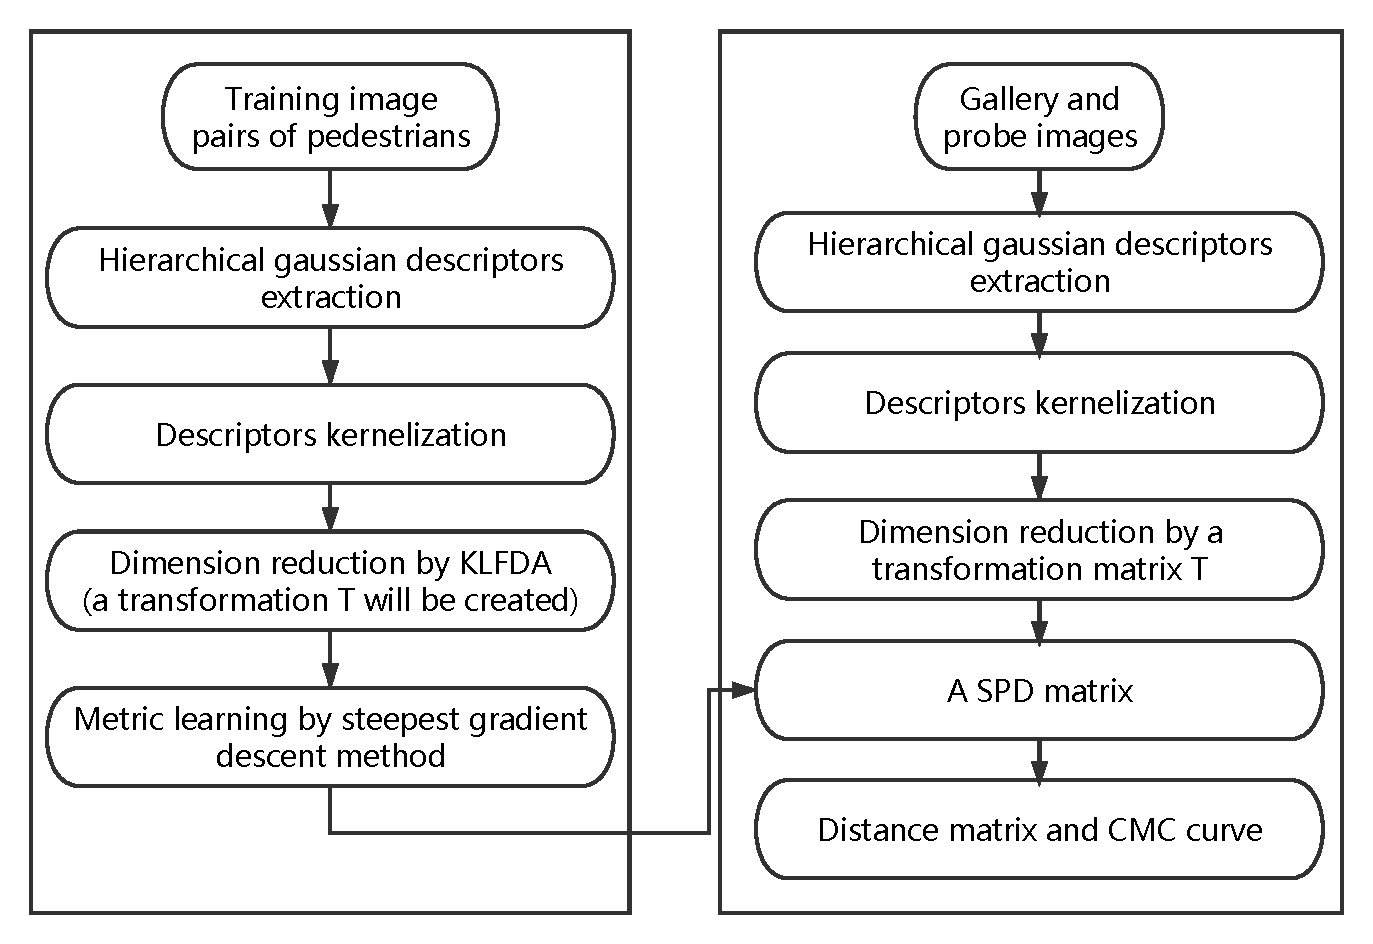
\includegraphics[width=1\linewidth]{/Users/JohnsonJohnson/Downloads/thesis_1/Figures/ProposedWorkFlow.pdf}
\vspace{-2em}
\caption{The workflow of proposed work; the left part is training and the right part is testing}
\label{ProposedWorkflow}

\end{figure}
%------------------------------------------------------------
\begin{figure}[H]

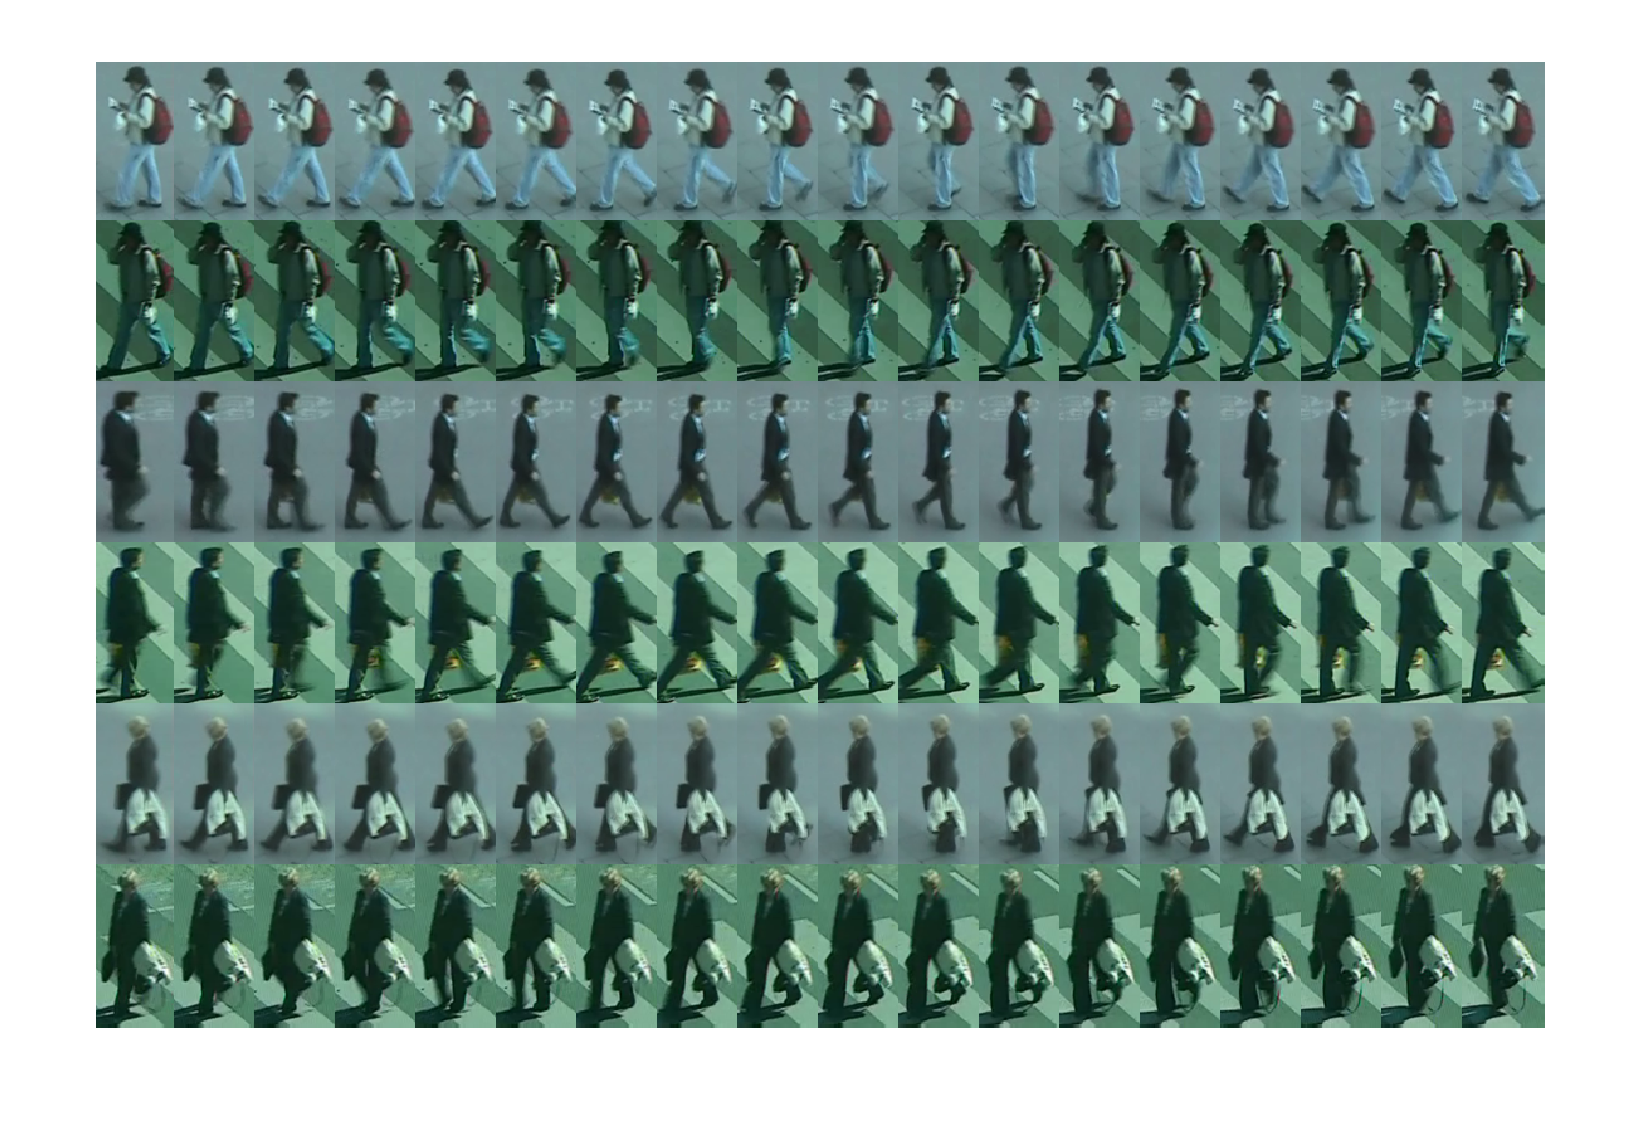
\includegraphics[width=1\linewidth]{/Users/JohnsonJohnson/Downloads/thesis_1/Figures/Multishots.eps}
\vspace{-2em}
\caption{Samples from the prid\_2011 dataset}

\end{figure}


\section{Contributions}

In this paper, we have three contributions. The first is that we combined the KLFDA with distance comparison metric learning. Instead of learning a subspace with KLFDA and computing Euclidean distance in the lower-dimensional space, in this thesis after dimension reduction by KLFDA a Mahalanobis metric is learned under the constraint that the maximum intraclass distance is at least one unit smaller than the minimum interclass distance. Compared with those advanced metrics including cross view quadratic analysis (XQDA) \cite{LOMO} and the null Foley-Sammon transfer (NFST), this proposed metric learning proves to have excellent performance on the VIPeR, CUHK1, prid\_2011, prid\_450s and GRID dataset.

Another contribution is we find that imperfect background subtraction increases histogram feature's performance and decreases textural feature's performance. Since in single-shot Re-ID, it's extremely hard to extract the foreground perfectly (only one frame of each individual is available to extract foreground), the extracted result may lose some parts of the foreground while contains some parts of the background. This imperfect foreground extraction can improve the performance of some descriptors, like the histogram of HSV color space, but can also decrease the performance of  other descriptors, like local binary pattern (LBP) and histogram of gradient (HOG). This comparison is shown in Chapter 3. The reason for this is that imperfect background segmentation brings in textural interference. If descriptors are color based and don't handle texture information, like HSV histogram descriptor, background segmentation can greatly improve the performance. However, if the descriptor extracts texture information, background segmentation will decrease its performance since the imperfect segmentation will mask out many parts of the foreground area, which will cause important textural information variation. Because segmentation algorithms will cause different influence on various features, in this thesis, a weighted map of images is used instead of the background segmentation.

For the last contribution, some variants of hierarchical Gaussian descriptor have been tested. In one variant, LBP was used in the basic pixel feature. In another variant, superpixel segmentation was also applied to combine with hierarchical Gaussian descriptor, which implied that overlapping patch sampling is important in the hierarchical Gaussian descriptor. At last, the Gaussian mixture model (GMM) was also tested but it displayed the worst performance.

\section{Thesis organization}
In this thesis, Chapter 2 will give a brief introduction of previous work. Chapter 3 will explain the implementation of the hierarchical Gaussian descriptors used in this thesis. This is also the chapter where my work starts. The performance of some variants of the hierarchical Gaussian descriptor is studied in this chapter. In Chapter 4, a detailed introduction of the kernel local Fisher discriminant analysis will be presented, and a detailed explanation of the metric learning on the lower-dimensional space based on relative distance limitation learning will also be provided.
In Chapter 5, the used datasets and parameters and other experiment settings will be explained, and a detailed analysis of results will be presented there. Finally, the conclusion is given in Chapter 6.




